\chapter{Methodology}
\label{ch:Methodology}

This work is applied research because it is designed to build a tool to solve an existing issue in the context of a real organization. The research will use a method for data analysis already established in the context of EDM problems, as it was described in section \ref{sc:edm}, where data will be collected, then DM algorithms will be applied to that data and, finally, a comparative analysis between those algorithms will be made. Because of this approach, it can be said that the research uses quantitative methods \cite{gomes2019classificaccao}.

Further, this research follows the procedure defined by Design Science Research\abrv{Design Science Research}{DSR}(DSR). DSR is commonly used when the researcher is interested in (1) solve a practical problem in a specific context through the development of an artifact, which is anything built to reach an objective; and (2) produce new knowledge. DSR is based on two cycles (1) design cycle, which aims to create an artifact, evaluate and refine the project; and (2) knowledge cycle, which aims to elaborate theoretical suppositions related to human behavior, that has phases such as validation, execution, analysis, and research contribution \cite{pimentel2019design}.

Following the objectives of DSR, this work aims to build a web system as a new software artifact and intends to create new knowledge about this research topic. Figure \ref{fig:dsr} presents the two cycles of DSR and how it is used by this research. It can be seen that the evaluation is based on three aspects: (1) if the artifact meets the requirements, (2) if the problem was successfully solved, and (3) if the theoretical conjectures seem valid.

\begin{figure}[htb]
	\centering
  	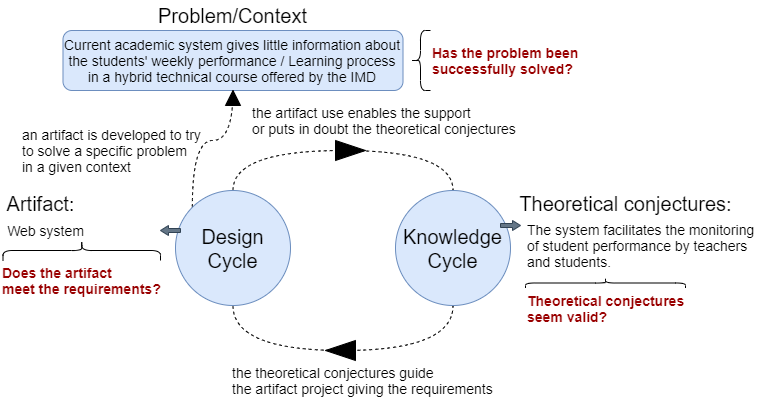
\includegraphics[scale=.55]{Imagens/dsr.png}
  	\caption{DSR process (adapted from \cite{pimentel2019design})}
  	\label{fig:dsr}
\end{figure}

The central objective of this research is to develop a web system for student performance prediction that helps with the learning process that the students from the IMD's IT technical course go through. This system will use DM techniques with the educational data provided by the Sistema Integrado de Gestão de Atividades Acadêmicas\abrv{Sistema Integrado de Gestão de Atividades Acadêmicas}{SIGAA}(SIGAA), which is the system used at IMD to manage the academic environment.

The main stakeholders associated with this research are the teachers and students of the IMD. It is hoped that the proposed web system can help teachers detect students that may require additional support, and give the students another way of monitoring their performance, thus, enhancing their academic experience.

The following sections present details about the data set, tools needed and a list of the project activities.

\section{Data set}

The data was requested to Superintendência de Tecnologia da Informação (STI), the university sector responsible for the SIGAA system, in early April 2021. Soon after, it was received a single report file in a comma-separated values file with all the required data. The structure of the data set is presented in appendix \ref{ch:Dataset}.

Before requesting the data a few project decisions were made, based on previous knowledge about the IMD's IT technical course structure: (1) work only with data from classes in the first semester of the course. This choice was made given how much more data is available relative to classes from the following semesters. (2) Use only data from the most recent curriculum, for the same reason as the previous decision. In addition, it was not requested any sensitive information about the students. This was done to preserve learners' information because of privacy regulations, and also because to achieve the goals of this research it is sufficient to use only data about scores and attendance of students.

The full data set has a total of 127 features and 6316 samples. The data ranges between years 2015 and 2020 and contains the scores and attendance of the students in all classes (6 in total), all weeks (up to 20 weeks), scores by different tasks (4 distinct types of tasks), and the final result in the first semester of the course. Details about the distribution of the samples through the years are shown in table \ref{tab:sbys}.

\begin{table}[htb]
\centering
\begin{tabular}{cc} \hline
\textbf{Semester} & \textbf{Number of samples} \\ \hline
2015.1 & 1351 \\
2016.1 & 1160 \\
2017.1 & 1076 \\
2017.2 & 697 \\
2018.1 & 639 \\
2019.1 & 634 \\
2020.1 & 759 \\ \hline
\end{tabular}
\caption{Amount of samples in the data set by semester}
\label{tab:sbys}
\end{table}

\section{Tools}

The data analysis step of the project was developed using Python\footnote[1]{\hspace{1mm}\url{https://www.python.org}} programming language and the Google Colaboratory\footnote[2]{\hspace{1mm}\url{https://colab.research.google.com}} environment. The Python language was chosen given the easiness of use and broad ecosystem available to solve DM problems. The libraries used are the following: pandas\footnote[3]{\hspace{1mm}\url{https://pandas.pydata.org}} and NumPy\footnote[4]{\hspace{1mm}\url{https://numpy.org}} (for data analysis and scientific computing), Matplotlib\footnote[5]{\hspace{1mm}\url{https://matplotlib.org}} and Seaborn\footnote[6]{\hspace{1mm}\url{https://seaborn.pydata.org}} (for data visualization) and scikit-learn\footnote[7]{\hspace{1mm}\url{https://scikit-learn.org/stable/index.html}} (for the machine learning algorithms).

The web system was also developed using Python. The server was built using Flask\footnote[8]{\hspace{1mm}\url{https://flask.palletsprojects.com/en/2.0.x/}}, a micro web application framework, and Jinja\footnote[9]{\hspace{1mm}\url{https://www.palletsprojects.com/p/jinja/}} as the template engine. The libraries used are: Flask-RESTful\footnote[10]{\hspace{1mm}\url{https://flask-restful.readthedocs.io/en/latest/}} (for building the mock\abrv{Application Programming Interface}{API}API server), requests\footnote[11]{\hspace{1mm}\url{https://docs.python-requests.org/en/master/}} (for queries to the API), Bootstrap-Flask\footnote[12]{\hspace{1mm}\url{https://bootstrap-flask.readthedocs.io/en/stable/index.html}} (for the templates of the web system's pages), and joblib\footnote[13]{\hspace{1mm}\url{https://joblib.readthedocs.io/en/latest/}} (to manipulate the DM models' files).

\section{Project activities}

Based on the EDM process, this research was developed according to the following tasks:

\begin{enumerate}
    \item Define the problem this work aims to solve, after an analysis of the current state of the virtual learning environment used by the students of the IMD.
    \item Obtain the raw educational data that will be used in the research.
    \item Apply preprocessing techniques in that data to reduce complexity and prepare the data to be effectively used by the DM algorithms.
    \item Research the DM algorithms that are commonly used in predictive systems.
    \item Analysis of those algorithms aiming to find the model with the best results for the given data.
    \item Develop a web system prototype to be used by teachers and students for the visualization of the likelihood the student has to pass the course.
\end{enumerate}